\section{Verwendete Bibliotheken}

\subsection{Wiring Pi}

Um auf die GPIO (General-purpose Input/Output) Schnittstellen des Raspberry Pi zugreifen zu können, haben wir die Bibliothek Wiring Pi verwendet. Um die Bibliothek mit dem Cross-Compiler verwenden zu können, haben wir diese zunächst unter dem Pi compiliert und anschließend die entsprechenden Header und .so-Dateien auf den Entwicklungsrechner kopiert.\\
\\
Zum Kompilieren der Bibliothek wurde folgendes Tutorial verwendet:\\
\hyperlink{https://projects.drogon.net/raspberry-pi/wiringpi/download-and-install/}{https://projects.drogon.net/raspberry-pi/wiringpi/download-and-install/}
\subsubsection{Verwendung}

Um die Lib verwenden zu können muss zunächst eine Setup Funktion aufgerufen werden. Darüber hinaus ist es notwendig, dass das Programm anschließend mit Superuser Rechten ausgeführt wird.\\
\\
Wir verwenden die Funktion wiringPiSetup(void). Diese Funktion gibt den Pins andere Nummern, als die ursprünglichen. Der Vorteil ist, dass die Nummern der Pins zwischen den verschiedenen Raspberry Pi Revisionen gleich bleiben, obwohl diese sich intern zwischen den Revisionen unterscheiden.\\
\\
Die folgende Tabelle zeigt die Nummern, welche Wiring Pi verwendet:\\
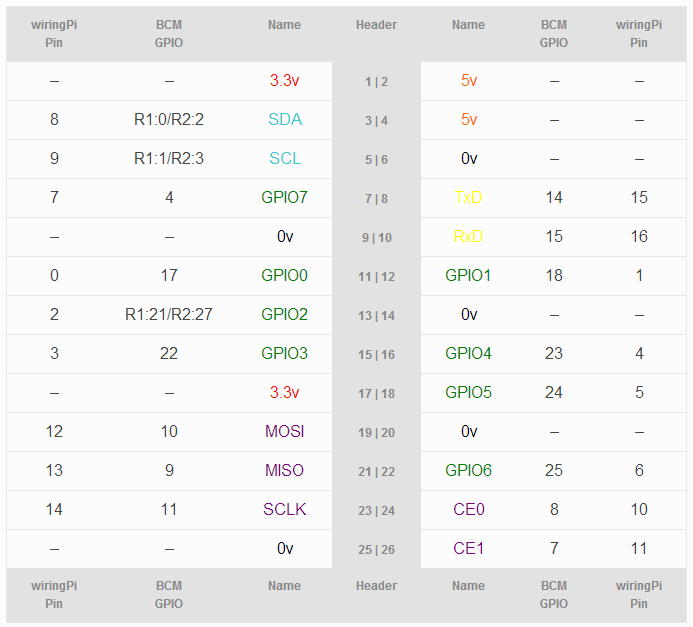
\includegraphics{GPIO_Pins.PNG}\\
\\
Um einen Pin ein- oder auszuschalten muss die Funktion digitalWrite genutzt werden. Der erste Parameter entspricht der Nummer des Pins und der zweite dem Status. Der Status kann "'HIGH"' (1) oder "'LOW"' (0) sein.\\
\\
Des Weiteren stellt die Bibliothek delay Funktionen zur Verzögung des Programms zur Verfügung.

\subsection{libmpdclient}
Um auf den mpd des Linux-Systems als Client zuzugreifen, verwenden wir eine Client-Bibliothek die sich "`libmpdclient"' nennt. Diese bietet die Möglichkeit, vorgefertigte Kommandos (z.B. Play und Pause) durch Aufrufen bestimmter Funktionen auszuführen oder direkt Befehle zum Server zu schicken. Diese können als String an eine Funktion übergeben werden.\\\\
Um die Bibliothek in unserem Projekt verwenden zu können, mussten wir zuerst die Bibliothek auf dem Raspberry Pi kompilieren, damit diese auf ARM Prozessoren funktioniert. Zum Kompilieren konnte ein Buildscript verwendet werden, welches mit der Bibliothek mitgeliefert wurde. Dieses Buildscript haben wir auf dem Raspberry Pi ausgeführt.
